\documentclass{mcmthesis}
\mcmsetup{CTeX = false,   % 使用 CTeX 套装时,设置为 true
        tcn = 2504959, problem = C,
        sheet = true, titleinsheet = true, keywordsinsheet = true,
        titlepage = false, abstract = true}
% \usepackage{newtxtext,newtxmath}
\usepackage{palatino}
\usepackage{lipsum}
\usepackage{lastpage}
\usepackage{graphicx}
\usepackage{epstopdf}
\usepackage{amsmath}
\usepackage{hyperref}
\usepackage{indentfirst}  % 引入宏包,使每个段落的首行缩进
\setlength{\parindent}{2em}  % 设置首行缩进的长度为2个字符

\title{Your Paper's Title(SHUMOJIAYOUZHAN)}
\bibliographystyle{unsrt}
\begin{document}
\begin{abstract}
% lipsum为随机生产的内容,这一部分为摘要,使用时把\lipsum[1]替换为你摘要的内容
\lipsum[1]
\cite{nosek2002math}


\begin{keywords}
keyword1; keyword2
\end{keywords}
\end{abstract}
\maketitle
%% Generate the Table of Contents, if it's needed.
 \tableofcontents
 \newpage
%%
%% Generate the Memorandum, if it's needed.


%%\section为一级标题,\subsection为二级标题 \subsubsection为三级标题

\section{Introduction}
% \begin{equation}
%   Z=a1+b1+c1+d1+e1+f1+g1+h1+i1+j1+k1+l1+m1+n1+o1+p1+q1+r1+s1+t1+u1+v1+w1+x1+y1+z1
% \end{equation}
\iffalse
这是一段被注释掉的内容。
这段文字不会出现在最终的输出中。
\begin{equation}
  \begin{split}
    Z=&a1+b1+c1+d1+e1+f1+g1+h1+i1+j1+k1+l1+m1+n1+o1\\
    &+p1+q1+r1+s1+t1+u1+v1+w1+x1+y1+z1
  \end{split}
\end{equation}
% \begin{itemize}……\end{itemize}为列表文本
\lipsum[2]
\begin{itemize}
% \item为要点强调,表现为黑色圆点
\item minimizes the discomfort to the hands, or 
\item maximizes the outgoing velocity of the ball.
\end{itemize}
We focus exclusively on the second definition.
\begin{itemize}
\item the initial velocity and rotation of the ball,
\item the initial velocity and rotation of the bat,
\item the relative position and orientation of the bat and ball, and
\item the force over time that the hitter hands applies on the handle.
\end{itemize}
\lipsum[3]
\begin{itemize}
\item the angular velocity of the bat,
\item the velocity of the ball, and
\item the position of impact along the bat.
\end{itemize}
\lipsum[4]
% 下述几种格式的效果可以去PDF里查看应用
\emph{center of percussion} [Brody 1986], \lipsum[5]
\begin{Theorem} \label{thm:latex}
\LaTeX
\end{Theorem}
\begin{Lemma} \label{thm:tex}
\TeX .
\end{Lemma}
\begin{proof}
The proof of theorem.
\end{proof}
\fi



\subsection{Problem Background}
During the Paris 2024 Summer Olympics, the medal table was the focus of fans, media and analysts around the world. The total number of medals won by each country not only measures the results of the competition, but also reflects the overall strength of each country's sports.

In the medal table, the performance of the traditional sporting powers is still remarkable. The United States topped the table with 126 medals, including 40 gold medals, 44 silver medals and 42 bronze medals, showing its strong competitiveness in many events. The Chinese delegation tied with the United States for the most gold medals with 40, but came second with a total of 91 medals. The host country, France, ranked fourth overall with 16 gold, 26 silver and 22 bronze medals, and fifth in gold medals, demonstrating its excellent performance at home.
Meanwhile, the performances of some of the smaller traditional sporting nations are also worthy of note. Dominica and Saint Lucia won their first Olympic medals at this year's Games, with Dominica taking gold. Countries such as Albania and Cape Verde have also achieved breakthrough results. Although the number of medals is small, these achievements are milestones in the Olympic history of these countries.

The dynamics of the medal table are also worth exploring. The number of medals won is a highly volatile, noisy, complex and unpredictable non-linear time series data. How to accurately predict a country's Olympic performance based on historical data, the number of gold, silver and bronze medals, “great coach” effect and other factors has become an important research topic.



\subsection{Restatement of the Problem}
\subsection{Our work}


\section{Analysis of the Problem}
% 

%插入图片 模板
\begin{figure}[h]
\small
\centering
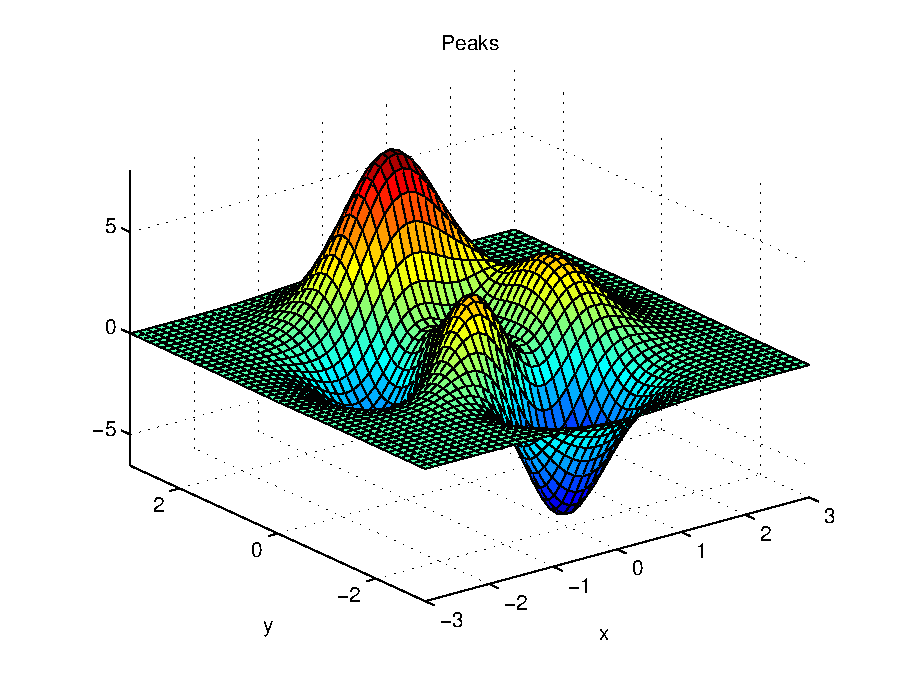
\includegraphics[width=12cm]{mcmthesis-aaa.eps}
\caption{aa} \label{fig:aa}
\end{figure}

\lipsum[8] \eqref{aa}

% \begin{equation}……\end{equation} 这种形式可以实现右编号
\begin{equation}
a^2 \label{aa}
\end{equation}
% \[   \]这种形式无编号
\[
  \begin{pmatrix}{*{20}c}
  {a_{11} } & {a_{12} } & {a_{13} }  \\
  {a_{21} } & {a_{22} } & {a_{23} }  \\
  {a_{31} } & {a_{32} } & {a_{33} }  \\
  \end{pmatrix}
  = \frac{{Opposite}}{{Hypotenuse}}\cos ^{ - 1} \theta \arcsin \theta
\]
\lipsum[9]

\[
  p_{j}=\begin{cases} 0,&\text{if $j$ is odd}\\
  r!\,(-1)^{j/2},&\text{if $j$ is even}
  \end{cases}
\]

\lipsum[10]

\[
  \arcsin \theta  =
  \mathop{{\int\!\!\!\!\!\int\!\!\!\!\!\int}\mkern-31.2mu
  \bigodot}\limits_\varphi
  {\mathop {\lim }\limits_{x \to \infty } \frac{{n!}}{{r!\left( {n - r}
  \right)!}}} \eqno (1)
\]

\section{Calculating and Simplifying the Model  }
\lipsum[11]

\section{The Model Results}
\lipsum[6]

\section{Validating the Model}
\lipsum[9]

\section{Conclusions}
\lipsum[6]

\section{A Summary}
\lipsum[6]

\section{Evaluate of the Mode}

\section{Strengths and weaknesses}
\lipsum[12]

\subsection{Strengths}
\begin{itemize}
\item \textbf{Applies widely}\\
This  system can be used for many types of airplanes, and it also
solves the interference during  the procedure of the boarding
airplane,as described above we can get to the  optimization
boarding time.We also know that all the service is automate.
\item \textbf{Improve the quality of the airport service}\\
Balancing the cost of the cost and the benefit, it will bring in
more convenient  for airport and passengers.It also saves many
human resources for the airline. \item \textbf{}
\end{itemize}

%\begin{thebibliography}{99}
%\bibitem{1} D.~E. KNUTH   The \TeX{}book  the American
%Mathematical Society and Addison-Wesley
%Publishing Company , 1984-1986.
%\bibitem{2}Lamport, Leslie,  \LaTeX{}: `` A Document Preparation System '',
%Addison-Wesley Publishing Company, 1986.
%\bibitem{3}\url{http://www.latexstudio.net/}
%\bibitem{4}\url{http://www.chinatex.org/}
%\end{thebibliography}
\bibliography{lit}

\newpage
\begin{appendices}

%  备忘录正文部分
%  \begin{memo}[Memorandum]
% 	\lipsum[1-3]
% \end{memo}


\section{First appendix}

\lipsum[13]

Here are simulation programmes we used in our model as follow.\\

\textbf{\textcolor[rgb]{0.98,0.00,0.00}{Input matlab source:}}
\lstinputlisting[language=Matlab]{./code/mcmthesis-matlab1.m}

\section{Second appendix}

some more text \textcolor[rgb]{0.98,0.00,0.00}{\textbf{Input C++ source:}}
\lstinputlisting[language=C++]{./code/mcmthesis-sudoku.cpp}


\newpage
\section{Report on Use of AI}
\begin{itemize}
\item OpenAI ChatGPT(Nov 5, 2023 version, ChatGPT-4)
\item Query1:Please briefly explain the common usages and main differences between RNN, GRU,LSTM.
\item Output: Recurrent Neural Networks (RNN), Gated Recurrent Units (GRU), and Long Short-Term  Memory (LSTM) networks are all types of neural networks designed to handle sequential data, such as
time series data, natural language text, and audio. They are primarily used in tasks that involve temporal
dependencies, where the order of the input data is crucial for making predictions or understanding
context. Common Usages RNN: Used for modeling sequence data but has limitations in learning
long-term dependencies due to the vanishing gradient problem. Commonly used in earlier applications
of language modeling and text generation. GRU: Introduced as a simpler alternative to LSTM with
fewer parameters. It is efficient in capturing dependencies for sequences of moderate length and is
used in tasks like speech recognition, language modeling, and text generation. LSTM: Specifically
designed to overcome the vanishing gradient problem of RNNs, making it capable of learning longterm dependencies. LSTMs are widely used in complex sequence modeling tasks, including machine
translation, speech recognition, and time series prediction. Main Differences Complexity: LSTMs are
more complex than GRUs, as they have three gates (input, output, forget) compared to GRU’s two
gates (update and reset). RNNs are the simplest, with no gates, leading to their inability to capture
long-term dependencies as effectively as GRU and LSTM. Memory Capability: LSTMs are best suited
for applications requiring the understanding of long-term dependencies due to their complex gating
mechanisms. GRUs are more efficient than LSTMs for shorter sequences but can still handle long-term
dependencies better than RNNs. Training Time and Parameters: Due to their simplicity, RNNs have
fewer parameters and thus are faster to train than GRUs and LSTMs. However, GRUs strike a balance
between complexity and performance, often requiring less training time than LSTMs due to having
fewer parameters, while still performing comparably on many tasks. Use Cases: The choice between
RNN,
  \end{itemize}
\end{appendices}



\end{document}

%% 
%% This work consists of these files mcmthesis.dtx,
%%                                   figures/ and
%%                                   code/,
%% and the derived files             mcmthesis.cls,
%%                                   mcmthesis-demo.tex,
%%                                   README,
%%                                   LICENSE,
%%                                   mcmthesis.pdf and
%%                                   mcmthesis-demo.pdf.
%%
%% End of file `mcmthesis-demo.tex'.
